%----------------------------------------------------------------------------------------
%	PACKETS AND CONFIGURATION
%----------------------------------------------------------------------------------------

\documentclass[11pt]{beamer}
\setbeamercovered{transparent}

\usepackage{title}  		% Title settings for the presentation
\usepackage{parskip}    	% Paragraph indent & skip
\usepackage{xcolor}     	% More colors
\usepackage{enumitem}		% Better lists
\usepackage{graphicx}  		% 'graphics' package interface
\usepackage{listings}   	% Code sections formatting}
%\usepackage{pdftexcmds}
%\usepackage{minted}
%\usepackage[utf8]{inputenc}
%\usepackage[T1]{fontenc}
%\usepackage{pythontex}
\usepackage{verbatim}

% Custom colors
\definecolor{AnnotationGreen}{RGB}{34, 128, 45}
\definecolor{CommentGreen}{RGB}{29, 204, 49}

% Python code formatting
% Use it by creating an environment like \begin{lstlisting}[style=Python] ... \end{lstlisting}
% Since annotations aren't tagged as keywords I have inserted a manual delimiter for them,
% it works as follows: \@@AnnotationText@@/
\lstdefinestyle{Python}{
    language = Python,
    basicstyle = \footnotesize\ttfamily,
    commentstyle = \textcolor{CommentGreen},
    stringstyle = \textcolor{orange},
    showstringspaces = false,
    keywordstyle = \textcolor{blue},
    moredelim = [is][\textcolor{AnnotationGreen}]{\\@}{@@\/},   % Annotations
    numberstyle = \scriptsize\ttfamily\textcolor{gray},
    numbers = left,
    frame = single,
    frameround = tttt,
    framexleftmargin = 10pt,
    framexrightmargin = 0pt
}

% HELPER PACKAGES (TODO: REMOVE IN FINAL) %
\usepackage{todonotes}
\presetkeys{todonotes}{inline}{}
\usepackage{blindtext}
% HELPER PACKAGES (TODO: REMOVE IN FINAL) %

\usetheme{Copenhagen} % THEME

%----------------------------------------------------------------------------------------
%	DOCUMENT
%----------------------------------------------------------------------------------------

\begin{document}

% TITLE
\frame{\titlepage}

% Table of Contents
\begin{frame}{Project}
    \tableofcontents[hideallsubsections]
\end{frame}

% Environment and Simulation ------------------------------------------------------------

\AtBeginSection[]
{
\begin{frame}{}
    \tableofcontents[sections={\thesection}]
\end{frame}
}

% ----------------------------------------

\section{Introduction}

%-----------------------------------------

\begin{frame}

\frametitle{Introduction}
\framesubtitle{Project scope}

The focus of this project is to optimize the budget allocated for the advertisement campaigns of 5 different items in order to maximize the profit of an e-commerce website that sells products to the public.
Each page has a primary product and some secondary products, each user that lands on a page has a possibility to buy the primary prodcut and/or proceed to one of the secondaries with a given probability, the process repeats.

\end{frame}


%-----------------------------------------

\begin{frame}

\frametitle{Introduction}
\framesubtitle{Project scope}

The optimization has to be perfomed on different scenarios and different algorithms.
We had to direct our focus on bandit algorithms combining Gaussian Process with Upper Confidence Bound and Thompson Sampling algorithms.
For each different scenario the performance of the learners based on these algorithm is evaluated against the Clayrvoiant and the Stupid Learner.

\end{frame}

%-----------------------------------------

\begin{frame}

\frametitle{Introduction}
\framesubtitle{General hypoteses}

The main general hypoteses that were given to us are:
\begin{itemize}[label={-}]
    \item For every primary product, the secondary products to display and their order is fixed.
    \item The price of every product is fixed and it is equal to the margin.
    \item By clicking a specific ad, the user lands on the corresponding primary product.
\end{itemize}

\end{frame}

% ----------------------------------------

\section{Environment and Simulator}

%-----------------------------------------

\subsection{Overview}

%-----------------------------------------

\begin{frame}

\frametitle{Environment and Simulator}
\framesubtitle{General hypotesis}

For this project, we are required to design an Environment that satisfies various constraints both on the e-commerce site's properties and on the users' behavior; in addition, since most of the tasks were generic, we had to come up with some of our own assumptions.
In particular we want to underline the following for the e-commerce website:
\begin{itemize}[label={-}]
    \item The website has unlimited units for the 5 different items.
    \item Actions on the webpages are perfectly observable by the ecommerce website.
\end{itemize}

\end{frame}

% ----------------------------------------

\begin{frame}

\frametitle{Environment and Simulator}
\framesubtitle{General hypotesis}

...and we assume that the users present the following behaviors:
\begin{itemize}[label={-}]
    \item Every day, there is a random number (subject to noise) of potential new users.
    \item The reservation price for each user is always over the single unit.
    \item The users can activate parallel paths while on the webpage.
    \item The number of items that a user will buy is a random variable, independent from any other variable.
\end{itemize}

\todo{insert text somewhere}
%The behavior of a user is modelled as a graph where nodes represent product pages and weights represent the probabilities for the user to click from the primary item of the page to one of the secondaries.

\end{frame}

%-----------------------------------------

\subsection{Environment structure}

%-----------------------------------------

\begin{frame}[fragile]

\frametitle{Environment and Simulator}
\framesubtitle{Environment}

The environment is modelled as a python dataclass containing the following attributes:

\begin{lstlisting}[style=Python, basicstyle=\tiny, numbers=none, framexrightmargin=-20pt]
    # The total budget to subdivide
    total_budget: int

    # Probability of every class to show up. They must add up to 1
    class_ratios: List[float]

    # Features associated to every class
    class_features: List[List]

    # Price of the 5 products
    product_prices: List[float]

    # List of class parameters for each class and product,
    # implemented as list of lists of UserClassParameters.
    # Each class has distinct parameters for every product
    classes_parameters: List[List[UserClassParameters]]
\end{lstlisting}

\end{frame}

% ----------------------------------------

\begin{frame}[fragile]

\frametitle{Environment and Simulator}
\framesubtitle{User classes}

We modelled the $\alpha$-functions, which compute the expected value of interactions on a product given a fixed budget, as exponential functions.
In particular their upper bound represents the maximum expected number of interactions possible while the maximum useful budget isthe amount of budget after which any budget increase would not lead to a ratio increase.


\begin{lstlisting}[style=Python, basicstyle=\tiny, numbers=none, framexrightmargin=-20pt]
    # Lambda parameter, which is the probability of osserving the
    # next secondary product according to the project's assignment
    lam: float

    # Max number of items a customer can buy of a certain product.
    # The number of bought items is determined randomly with
    # max_items as upper bound
    max_items: int

    # Products graph's matrix. It's a empty matrix, should be
    # initialized with populate_graphs
    graph: np.ndarray

    # List that constains for every i+1 product the secondary i+1
    # products that will be shown in the first and second slot
    next_products: List[Tuple[int, int]]

    # Controls randomness of the environment
    random_noise: float
\end{lstlisting}

\end{frame}

% ----------------------------------------

\begin{frame}

\frametitle{Environment and Simulator}
\framesubtitle{User classes}

\begin{itemize}[leftmargin=*, label={$\circ$}]
    \item Users are subdivided in classes based on their 2 binary features for a total of 3 different classes.
    \item In particular, each user class is defined by its $\alpha$-functions (one for each product plus the one for the non-strategic competitor) which define the probability of landing on a given product page.
    \item Each $\alpha$-function is defined by the values: \textbf{reservation price}, \textbf{upper bound} and \textbf{maximum useful budget}
\end{itemize}

\todo{alpha functions aren't sigmoidal! we changed to the exponential function - correct and move to a new slide maybe}
%Since the $\alpha$-functions we had choosen belong to the sigmoidal class we need these additional parameters.
%\begin{figure}[⟨r⟩]
%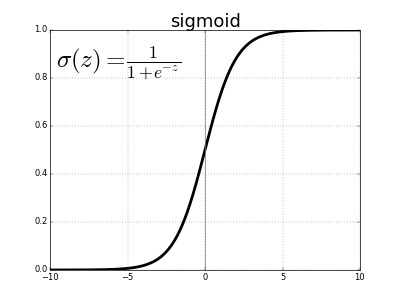
\includegraphics[height=3.8cm]{img/Graphs/sigmoid.png}
%\end{figure}

\end{frame}

% ----------------------------------------

\begin{frame}

\frametitle{Environment and Simulator}
\framesubtitle{Masked Environment}

Alongside the Environment we define a Masked Environment with the purpose of hiding crucial information to the learners since each type of learner should only have access to a subset of all the information available in the environment dictated by the type of learner.

The masked environment isn't strictly needed in the project since the learners could easily ignore the extra information, however, we wanted to face the problem with an approach aimed towards reusability and extendability and in this case (as in many others down the line) we opted for a more generalizable solution.

\todo{we talk about learners without metioning them before, we need to introduce them in the introductory section}

\end{frame}

% ----------------------------------------

\subsection{Randomness in the Environment}

% ----------------------------------------

\begin{frame}

\frametitle{Environment and Simulator}
\framesubtitle{Randomness in the Environment}

\begin{itemize}[leftmargin=*, label={$\circ$}]
    \item For the sake of representing a real scenario, most of the values that are not known a priori are randomly generated and every variable that evolves through time without our direct control has elements of randomness to it (for instance, each day we randomly get the number of active total users in our scenario by using a gaussian distribution with tunable mean and standard deviation).
    \item Even though most of the randomness is tunable and controlled through seeded generators, there are still impactful elements of non determinism (i.e. the Dirichlet distribution) that are not possible to control in any way.
\end{itemize}

\end{frame}

% ----------------------------------------

\begin{frame}

\frametitle{Environment and Simulator}
\framesubtitle{Example of Environment}

We see here an example of environment initialization:
\todo{improve legibility}


%\begin{figure}[<t>]
%   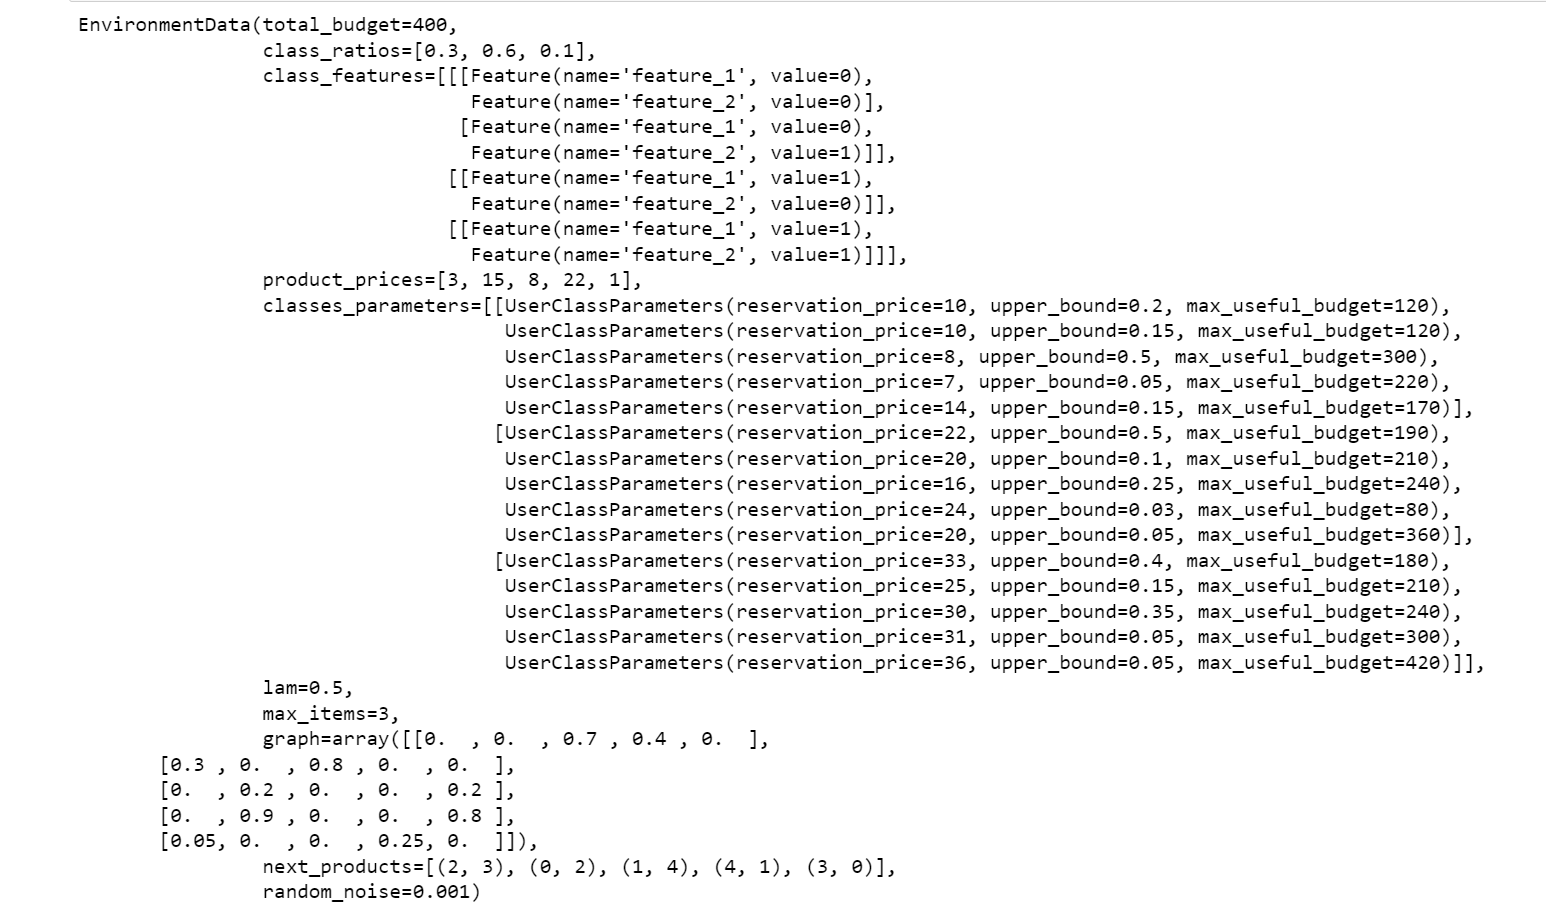
\includegraphics[height=6cm]{img/Graphs/Example_environment.png}
%\end{figure}

\end{frame}

% ----------------------------------------

\subsection{Simulation}

% ----------------------------------------

\begin{frame}

\frametitle{Environment and Simulator}
\framesubtitle{Daily Simulation}

\begin{itemize}[leftmargin=*, label={$\circ$}]
    \item The Simulation class is the main engine that brings together learner and environment by making them interact with each other while offering an interface to customize the execution.
    \item The basic idea of the simulation is to simulate a real scenario day by day using the environment to generate interactions with the website according to the budgets that the current learner proposed and then, feed the results back to the learner to make it actually learn.
    \item Repeating the simulation execution step for each day until an arbitrary time horizon is reached grants us all the data needed to evaluate the performance of our learner.
\end{itemize}

\end{frame}

% ----------------------------------------

\begin{frame}

\frametitle{Environment and Simulator}
\framesubtitle{Daily Simulation}

\todo{insert generic learner execution plot over n days}

\end{frame}

% Optimization Algorithm ----------------------------------------------------------------

\AtBeginSection[]
{
\begin{frame}{}
    \tableofcontents[sections={\thesection}]
\end{frame}
}

% ----------------------------------------

\section{Optimization Algorithm}

% ----------------------------------------

\subsection{General Problem}

% ----------------------------------------

\begin{frame}

\frametitle{Optimization Algorithm}
\framesubtitle{Problem Formulation}

The purpose of the optimization algorithm is to find the optimal budget for each campaign in order to maximize the profit, which is defined as the difference between the profits gained from selling products and the advertisement expenses.
Basically, it is the maximization problem subject to an obvious constraint: the sum of the daily budget can't be greater then the overall budget.

The optimization problem can be expressed as follows:
\begin{displaymath}
F=\max_{\substack{x_i\in B}} \sum_{i=0}^n \alpha_i(x_i)p_i-x_i \ s.t. \sum_{i=0}^n x_i\leq B
\end{displaymath}

\end{frame}

% ----------------------------------------

\subsection{Algorithm}


\begin{frame}

\frametitle{Optimization Algorithm}
\framesubtitle{}
\todo{talking about the code in words}

\end{frame}

% ----------------------------------------

\begin{frame}

\frametitle{Optimization Algorithm}
\framesubtitle{}
\todo{snippets of code}

\end{frame}

% Uncertain alpha functions -------------------------------------------------------------

\AtBeginSection[]
{
\begin{frame}{}
    \tableofcontents[sections={\thesection}]
\end{frame}
}

% ----------------------------------------

\section{Uncertain $\alpha$-functions}

% ----------------------------------------

\subsection{Contextual hypotesis}

% ----------------------------------------

\begin{frame}

\frametitle{Uncertain $\alpha$-functions}
\framesubtitle{Scenario}

We assume now that the binary features of the users cannot be observed and therefore data are aggregated.

\end{frame}

% ----------------------------------------

\subsection{Algorithm}

% ----------------------------------------

\begin{frame}
\frametitle{Uncertain $\alpha$-functions}
\framesubtitle{Algorithm}

Since the feature of the users are \textbf{not observable}, the algorithm receives all the interactions minus the class data.
It tries to estimate the reward given by each single product.

\end{frame}

% ----------------------------------------

\begin{frame}

\frametitle{Uncertain $\alpha$-functions}
\framesubtitle{Result}
\todo{: going to insert some graph of clayrvoiantv stupid}

\end{frame}

% Uncertain alpha functions and number of items sold ------------------------------------

%\section{Uncertain $\alpha$-functions and number of items sold}

% Uncertain graph weights ---------------------------------------------------------------

%\section{Uncertain Graph Weights}

% Non-stationary demand curve -----------------------------------------------------------

%\section{Non-stationary demand curve}

% Context generation --------------------------------------------------------------------

\AtBeginSection[]
{
\begin{frame}{}
    \tableofcontents[sections={\thesection}]
\end{frame}
}

% ----------------------------------------

\section{Context Generation}

%-----------------------------------------

\subsection{General Remarks}

%-----------------------------------------

\begin{frame}

\frametitle{Context Generation}
\framesubtitle{Basics}

The goal of \textbf{context generation} and \textbf{contextual bandit algorithms} is to employ a (partially) disaggregated approach in order to better exploit the differences of the users that belong to different classes.

This is made possible by using a specialized Learner for each context and an \textit{offline context generation algorithm} that decides which contexts are worth to target by isolating them from the aggregated data.

Each context is able to target a set of features, and a \textbf{context structure} is a set of contexts that targets all the existing features without any overlap.

\end{frame}

%-----------------------------------------

\begin{frame}

\frametitle{Context Generation}
\framesubtitle{}

\todo{todo}

\end{frame}

%-----------------------------------------

\subsection{Assumptions}

%-----------------------------------------

\begin{frame}

\frametitle{Context Generation}
\framesubtitle{Implementation challenges}

Context generation has been, by far, the \textit{toughest} task that we faced on this whole project.

Even after many meetings and discussions we felt that there was something that didn't click with our interpretation since we didn't find a way to give a complete meaning to the dataset collected by our active bandits due to how the prediction and the rewards worked in our scenario.

In the end, our final results for this step were \textbf{unsatisfactory} and there is still wide room for improvement.

\end{frame}

%-----------------------------------------

\begin{frame}

\frametitle{Context Generation}
\framesubtitle{Compromises}

Given the difficulties that we encountered, we decided to make some compromises in order to still carry out the task to an end:

\begin{itemize}[label={-}]
    \item The e-commerce website company owns a simulation capable of simulating interactions.
    \item Learners are trained on the fake simulation since we can't get enough information from the logs.
    \item The best expected reward for a given context is considered as the maximum reward experienced by a learner on a fake simulation run.
    \item We used the Hoeffding bound to calculate lower bounds for both the probability and the best expected reward for the contexts
\end{itemize}

\end{frame}

%-----------------------------------------

\subsection{Implementation}

%-----------------------------------------

\begin{frame}

\frametitle{Context Generation}
\framesubtitle{Generation}

We generate contexts following a \textbf{greedy algorithm} that, given a context $c$:

\begin{itemize}[label={*}]
    \item Considers all the possible binary 1-feature splits $\{c_i^0$, $c_i^1\}_n$ for the features not present in $c$.
    \item Creates and evaluates a new learner for each split $c_i^j$, obtaining the \textbf{context probability} $p_i^j$ and the \textbf{best expected reward} $\mu_i^j$.
    \item Evaluates the \textbf{splitting condition} on each couple of splits $(c_i^0$, $c_i^1)$ w.r.t the original context $c$ while deciding which split is the best one (if it exists).
    \item If a split has been made, repeat all the operations recursively on the new contexts until \textit{no split is made} or \textit{no split is possible}.
\end{itemize}

\end{frame}

%-----------------------------------------

\begin{frame}

\frametitle{Context Generation}
\framesubtitle{Split condition}

Since utilizing multiple contexts is an expensive operation and our \textit{greedy algorithm} is \textbf{not} guranteed to find the optimal solution, we want to be sure that when we introuduce new contexts, it is actually worth to do so.

We use a particular \textit{splitting condition} that exploits lower bounds in order to set a higher threshold for the quality of our splits:

\begin{Large}
    \begin{displaymath}
        \underline{p}_i^0 \underline{\mu}_i^0 + \underline{p}_i^1 \underline{\mu}_i^1 \geq \underline{\mu}_i
    \end{displaymath}
\end{Large}

\end{frame}

%-----------------------------------------

\begin{frame}

\frametitle{Context Generation}
\framesubtitle{Utilization}

Once a certain number of contexts has been established, a \textbf{Contextual Learner} will be able to assign an \textbf{Alphaless Learner} to each context and obtain their raw predictions by utilizing the function \textbf{predict\_raw} (which returns an un-optimized array of predictions) and then running the optimization algorithm on all the predictions gathered this way.

The resulting \textit{superarm} is then passed to the \textbf{Simulation} which, in return, generates the interactions for the day by weighting the different classes according to the disaggregated predictions.

\end{frame}

%-----------------------------------------

\subsection{Results}

%-----------------------------------------

\begin{frame}

\frametitle{Context Generation}
\framesubtitle{Results}

\todo{Insert results}

\end{frame}

%-----------------------------------------

\end{document}


%NOTE TO US:
%%\centering if we want the presentation to be power-point style
